\documentclass{article}
\usepackage[margin=2.2cm]{geometry}
\usepackage{graphics}
\usepackage{graphicx}

\usepackage{titlesec}
\usepackage{lipsum}
\usepackage{caption}
\usepackage{subcaption}

\begin{document}
	\section{CPP}
	Controllers can be placed in a Software Defined Network before or after clustering. The questions that need to be answered to place controllers efficiently can be as follows:
	\subsection{How many controllers?}
	Based on which criteria should the number of controllers be decided? It can be latency, response time, reaction time, etc. However, \cite{cpp2012heller} surprisingly found out that one controller is enough for a medium sized network. Increasing the number of controllers can decrease the average latency significantly. Three controllers can reduce the latency to half of that for one controller, while the same reduction in worst case latency requires four controllers. Assuming only optimization of one metric at the expense of the other, the point of diminishing returns? For a specific network (Internet2 OS3E topology), Heller et. al. shows that around 3-4 controllers does the job. Independently, Internet2 operators suggested a (3+1)-controllers setup as a reasonable starting point. Having three controllers and an extra one for fault tolerance. Therefore, we can conclude that while placing controllers for the first time, latency and fault tolerance are more important than load balance, as the load generated for a network with controllers will be available after the placement of controllers.
	
	\subsection{Where to place them?}
	Latency minimization can be broken down into two major categories such as: controller to controller latency and switch to controller latency. However, a standard controller placement algorithm should have the ability to place controllers based on whether controller to controller or controller to switch communication is more important. Therefore, we hope to provide a latency based solution in section \ref{latencyBased} which can place controllers considering both controller to switch and inter controller latencies.
	
	The placement metrics in \cite{cpp2012heller} are average-case latency and worst-case latency, which are calculated considering controller to switch latency. The algorithm does an exhaustive search for controller positions, placing \textit{k} controllers in all possible combinations. As a result the complexity increases exponentially for larger number controllers. Being a brute force algorithm, it ensures accurate result for the cost of high complexity and ignores controller to controller latency. To propose a more efficient algorithm, we have to propose a faster algorithm which minimizes both controller to switch and controller to controller latency as per requirement.
	
	\subsection{Which switch falls under which controller?}
	After the controllers are placed, changing their position physically becomes a challenge. However, the switches can be assigned to any controller while the network is still active. Dynamic assignment of switches can be based on load and controller reaction time, as latency is already address while placing controllers and link bandwidth is static. Therefore, we hope to propose an algorithm in section \ref{loadBased} which can balance load with minimum complexity so as to not put too much pressure on the already engaged controllers. The latencies must also be considered so that no switch is assigned to a far away controller when another controller is already close by.
	
	\section{Latency Based Controller Placement} \label{latencyBased}
	Our work in \cite{aziz2019degree} uses node degree to determine cluster heads in a unweighted graph and places controller again based on average inter-controller and intra-controller latency. However, the latter controller selection invalidates the selection of cluster heads based on unweighted degree.
	
	The latency for sending a data packet can be divided into four categories:
	\begin{itemize}
		\item \textbf{Propagation Latency:} The time required for the first bit of a data packet to traverse the link and reach the destination from the source is called the propagation latency. For example, the network Aarnet has switches distributed throughout Australia. The diameter of Australia is about \textit{4000 km} and data travels at the speed of light or close to the speed of light which is  \textit{300000 kmps}. Therefore, for a data packet traversing any link in Australia should require at most $\frac{4000}{300000}$ or $0.01333..$ seconds.
		\item \textbf{Transmission Latency:} This latency is the time required to send the packet starting from the first bit to the last bit into the medium of transport. This depends on bandwidth of the link as the bandwidth determines how much data can be converted to signals at the same time.
		\item \textbf{Processing Latency:} This latency is the amount of time required to decide which packet will be sent where. In case of SDNs, this is the time required for the switch to inform the controller and get a response for new flows and the time for flow matching of old flows.
		\item \textbf{Queuing Latency:} This delay is caused when traffic arrives faster than it can be processed and is affected by both transmission latency and processing latency. This is the time a packet needs to wait in the \textit{buffer} or \textit{queue} of a switch.
	\end{itemize}

	When a packet arrives at a switch, depending on the status of the switch, the packet is either kept in buffer/queue or processed immediately. Queuing delay is minimum when new packets are processed immediately, as a consequence of faster processing and transmission. When the packet is processed, it is either matched with an existing flow or in the case of a flow mismatch, the appropriate controller is sent a query message. After processing, the packet is transmitted into the medium for delivery to the intended destination. The speed of transmission is dependent on the link bandwidth and the processing delay is determined by the flow table management. Therefore, in our experiments, we consider latency (an inverse relation of bandwidth) as the weight of the edges connecting the switches.
	
	The controller of a network should have the ability to communicate with switches as fast as possible to minimize queuing latency and improve overall network throughput. Consequently, the controller should be the nearest to all the switches of the network, meaning -- the controller should be at the center of the network. However, for multiple controllers the placement becomes a bit more tricky. The placement should reflect the priority of controller to controller communication as per requirement. Based on the priority of inter-controller communication, we use a normalized priority constant when placing controllers in a cluster. We place controllers after clustering the network into our required number of sub-networks to place controllers. This clustering is only done to place controllers evenly throughout the entire network. The assignment of switches can change according to load (explained in section \ref{loadBased}). We experiment with our previous algorithm with changed inputs like weighted networks and check the placements manually.
	
	\subsection{Formulation of Latency Based Solution}
	Our proposed algorithm in progress consists of the following steps (in detail):
	\begin{enumerate}
		\item We calculate all pair shortest paths considering latency as the distance between each connected switch pair.
		
		\item We find the best position for a controller in a single controller network. Using both average case latency and worst case latency as metric, we select the center of the network Aarnet (Figure \ref{fig:aarnet2009}). We observe that average case latency gives a better placement for a single controller (Figure \ref{fig:aarnet2009mod}).
		
		\item For multiple controller placement, the center can act as the reference as it has the maximum probability to be at the border of the clusters or at the center of a cluster when the sub-networks are balanced. For two controllers, the network should ideally be divided into two equal sub-networks, for three controllers, three sub-networks and so on.
		
		\item We select multiple \textit{cluster-heads} like our previous algorithm for each cluster. However, we rename them as \textit{cluster-center} as we will select cluster-centers for the sole purpose of equal division of the network and not controller selection. In DBC (our previous algorithm) we use degree as selection criteria for cluster head, which makes sense when selecting controllers. However, for selecting cluster heads or \textit{cluster-centers}, we require a more deterministic criteria instead of a partially random one like degree. We use average distance from other nodes as the selection criteria of cluster-centers. The nodes will be sorted in ascending order of average distance, where we observe that the order also represents the distance from the center (unless a far away node has better connectivity). Therefore, if the nodes from the list are selected maintaining a distance of cluster radius ($T_d$) then the resulting nodes will be better candidates for cluster center (node degree only represented one hop connectivity).
		
		\item In our new algorithm Latency-based Balanced Clustering (LBC) instead of maintaining cluster radius ($T_d$) we use Breadth First Search (BFS) to directly find the number of nodes to cluster for a particular sub-network. If the number of remaining clusters is $k$ and the total number of nodes left to cluster is $n$, then the number of nodes per cluster is $n/k$.
		
		\item Our first attempt at using BFS to cluster a network from cluster center created stray nodes and made the clustering a bit jumbled (Figure \ref{fig:aarnet2009bfs}). We use Dijkstra next and the result is still not satisfactory as the bandwidth of the links is given a very high priority due to their higher numerical differences(Figure \ref{fig:aarnet2009Dijkstra}). There also seems to be higher cases of isolated nodes or islands.
		
		\item We learn from our previous experiments that the cluster-centers are still the same for both the clustering and we conclude that assigning nodes to the cluster-centers erroneous. Therefore, we select the cluster-centers using bfs and assign the nodes closest to each cluster-center using distance (or latency) as metric. Although latency values greatly vary from node to node, it is still efficient when assigning switches by comparing the distance of a switch to all controllers.
		
		\item When increasing cluster size from cluster-center, we expand hop by hop until \textit{n/k} nodes are clustered. Then we decrease average latency of the remaining nodes by subtracting the distances from the already clustered nodes. After selecting \textit{k} cluster-centers in this way, we assign switches based on weighted distances to form clusters.
		
		\item We select controllers based on our previous algorithm DBC by calculating average controller to switch distance ($intraController$) and approximated controller to controller distance ($interController$) and prioritizing each latency with a constant ($\alpha$).
	\end{enumerate}
 
 	\begin{figure}
 		\centering
 		\begin{subfigure}[b]{0.45\textwidth}
 			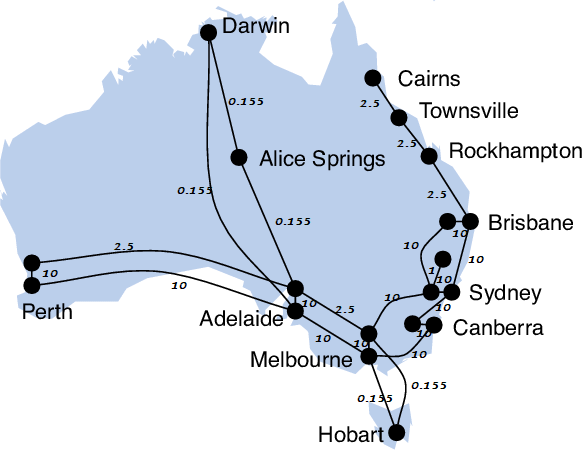
\includegraphics[width=\linewidth]{Images/aarnet2009.png}
 			\caption{Original Network with Link Bandwidth}
 			\label{fig:aarnet2009}
 		\end{subfigure}
 		~
 		\begin{subfigure}[b]{0.45\textwidth}
 			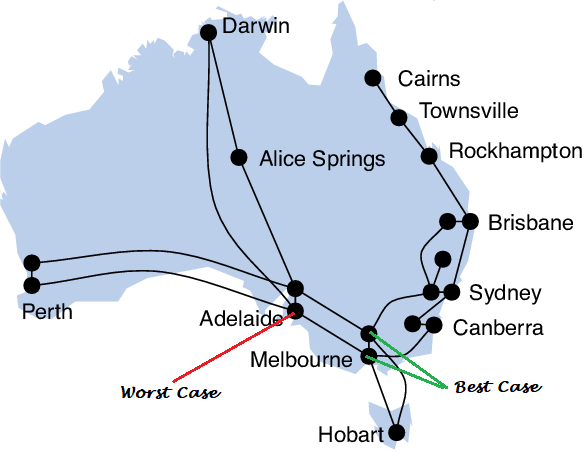
\includegraphics[width=\linewidth]{Images/aarnet2009mod.png}
 			\caption{Network after placing one controller}
 			\label{fig:aarnet2009mod}
 		\end{subfigure}
 		~
 		\begin{subfigure}[b]{0.45\textwidth}
 			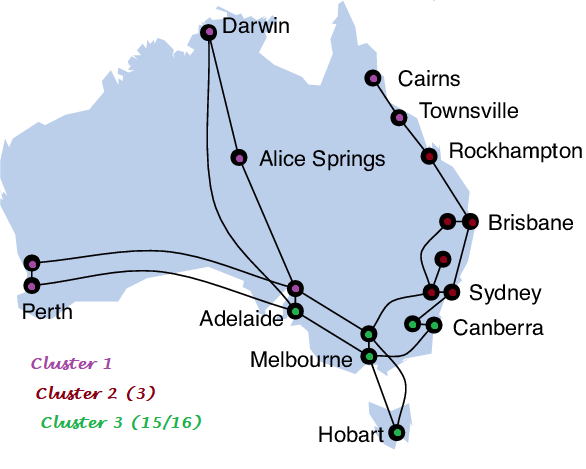
\includegraphics[width=\linewidth]{Images/aarnet2009_with_bfs.png}
 			\caption{Network after applying LBC using BFS}
 			\label{fig:aarnet2009bfs}
 		\end{subfigure}
 		~
 		\begin{subfigure}[b]{0.45\textwidth}
 			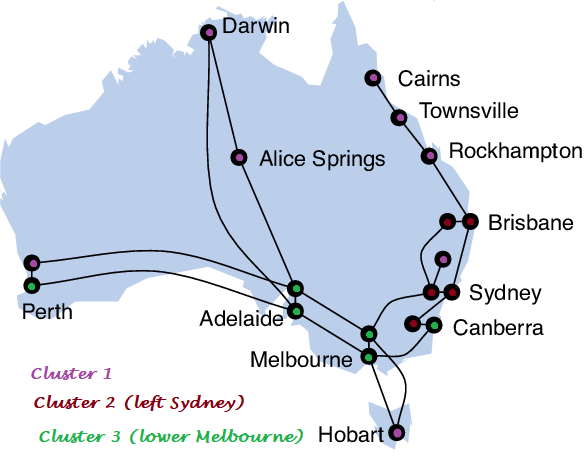
\includegraphics[width=\linewidth]{Images/aarnet2009_with_dijkstra.png}
 			\caption{Network after applying LBC using Dijkstra}
 			\label{fig:aarnet2009Dijkstra}
 		\end{subfigure}
 		\caption{Existing network of Australia, collected in 2009 and updated last in 2011}
 	\end{figure}
	 
	\subsection{Performance Evaluation}
	We use the following performance metric to determine the overall latency of the network:
	\begin{equation} \label{eqn:setupLatency}
	\Omega(S) = \frac{2}{|S|\times |S-1|}\sum_{s_i,s_d\in S} \{dis(s_i,c_i)+\\ \max_{s_j\in path_{i,d}}\left(dis(c_i,c_j)+dis(c_j,s_j) \right) \}
	\end{equation}
	
	here, $path_{i,d}$ is the shortest path from source switch $s_i$ to destination switch $s_d$, $c_i$ and $c_J$ are their respective controllers and $S$ is the network.
	
	The evaluation metric is same as in our previous work \cite{aziz2019degree} and our previous target paper \cite{dbcp2017}. When a new flow is detected in a switch to be sent to another switch, the controller is notified. The controller then notifies all the switches of the new path directly or through other controllers for the new flow. Minimizing this latency through proper controller placement determines the effectiveness of the placement algorithm. Therefore, the average of all pair to pair latencies $\Omega(S)$ gives the overall latency of the network $S$.
	
	\section{Load Based Solution} \label{loadBased}
	The initial load based solution \cite{yao2014capacitated} proposed three main reasons for considering the loads of controllers when placing controllers.
	\begin{enumerate}
		\item \textbf{The server capacity limitation.} The server has limited resources to manage a limited number of routers.
		\item \textbf{The latency of message of processing.} When the controller capacity threshold is reached, the message processing latency increasing substantially.
		\item \textbf{Failure.} Heavy-load controllers have higher failure probability as they have less resources to handle errors and attacks.
	\end{enumerate}

	Observing the experimental setup, we came up with the following parameters while working with an SDN:
	\begin{itemize}
		\item \textbf{Flow Generation Rate of Network:} $400000 \times N$ per second where $N$ is the number of routers.
		\item \textbf{Server NIC access bandwidth:} maximum 10 Gbps, and assuming each controller runs on a single server, the controller has the same bandwidth.
		\item \textbf{Flow mismatch packet entry rate:} 7.8 Mpps (million packets per second), where each packet is on an average 160 byte, resulting in $10G/(8\times 160)$ pps (packets per second) possible at max
	\end{itemize}
	Based on these calculations, for each 20 routers approximately 1 controller is needed to respond to the generated load completely, assuming that each controller has access bandwidth equivalent to 10Gbps. However, this is only for the best case scenarios where each controller can handle maximum load and the load is equally distributed.

	Observing the above specifications, we can conclude that the load of the network need to be distributed properly for proper functioning of the controller and to avoid increased processing latency.
	
	\subsection{Heuristic Search}
	Dynamic assignment of switches to controllers in a live network can keep the load of the network balanced. However, only balancing loads will not ensure maximum throughput of the network as assigning switches faraway can increase latencies instead decreasing it. For example, in the previous network if we assume a given load of switches, assume that each controller has identical processing capacity and assign switches to controllers as given in figures 1 and 2, we can observe the following:
	\begin{itemize}
		\item The load of the network in Figure 1, is balanced ideally as each controller gets $L/k$ load where $L$ is the total load of the network and $k$ is the number of controllers.
		\item Switches are assigned to far away controllers in figure 1 to maintain an ideal distribution of load.
		\item Although the load is balanced for controllers, some switches have more traffic than required in Figure 1 (mention switches). This results in decreased throughput and increase overall latency of the network.
		\item The distribution of load in Figure 2 prioritizes distance over load balancing, as a result, there are no overlapping of clusters under any controller.
	\end{itemize}
	Keeping the above mentioned points in mind, we work with nodes bordering a cluster instead of all the nodes and we start with an already clustered network (based on latency) to avoid unnecessary processing. There we express the load balancing problem as a heuristic based optimization problem with the following foundations:
	\subsubsection{Initial State}
	The initial state of the network is the assignment of switches to controllers according to the Latency Based Solution (section \ref{latencyBased}).
	
	\subsubsection{Current State}
	The current state can be the initial state of the network, or the modified state of the network where the assignment of switches to controllers is different than that of the initial state.
	
	\subsubsection{Target State}
	The target state of a network $S$ containing $k$ controllers and total load of $L$ is a distribution of load through assignment of switches so that each controller has load of $\frac{L}{k}$. Although this state may very well be unreachable in some cases, an approximation (with least error) closest to the target state must be attained.
	
	\subsubsection{Error Function}
	The error function is the squared sum of the differences of all controller loads and average load ($\frac{L}{k}$). Squaring the differences gives more priority to controllers whose loads are more imbalanced then others compared to a collective imbalanced load. If load of each controller is $l_1$, $l_2$,.. and so on, then the calculated error of the state is $[(l_1-\frac{L}{k})^2 + (l_2-\frac{L}{k})^2 + ..... + (l_k-\frac{L}{k})^2]/2$. As the extra loads of a controller is repeated for one or more under-loaded controllers, we decrease the error function to its half.
	
	\subsubsection{Next/Adjacent State(s)}
	The next states of the current state is the assignment of a border node of a cluster under a controller to a neighboring cluster under a different controller. All such combinations constitute the set of adjacent states.
	
	\subsubsection{Heuristic}
	This is a bit challenging as a greedy solution may reach a local optimal solution but might not find the target or optimal solution. However, if there is no optimal solution, then the sub optimal solution might be the best one. The most simple form of heuristic could be the error according to the above mention error function. In that case, the adjacent state with the least error is the best option.
	
	We attempt to use \textbf{BestFS} (best first search) algorithm to find the best solution. We do not want a perfectly balanced load, rather we want an assignment of nodes which keeps variation within a specific limit and does not produce unwanted traffic due to overlapping of clusters.
	
	\section{Conclusion}
	
	\bibliographystyle{IEEEtran}
	\bibliography{mybib}
\end{document}